\FChapter{Chapter Thirty-Four}{34}

\Lettrine{I}{t} \textsc{was near Christmas} by the time all was settled: the season of general
holiday approached. I now closed Morton school, taking care that the
parting should not be barren on my side. Good fortune opens the hand as
well as the heart wonderfully; and to give somewhat when we have largely
received, is but to afford a vent to the unusual ebullition of the
sensations. I had long felt with pleasure that many of my rustic
scholars liked me, and when we parted, that consciousness was confirmed:
they manifested their affection plainly and strongly. Deep was my
gratification to find I had really a place in their unsophisticated
hearts: I promised them that never a week should pass in future that I
did not visit them, and give them an hour's teaching in their school.

\Mr{} Rivers came up as, having seen the classes, now numbering sixty
girls, file out before me, and locked the door, I stood with the key in
my hand, exchanging a few words of special farewell with some half-dozen
of my best scholars: as decent, respectable, modest, and well-informed
young women as could be found in the ranks of the British peasantry. 
And that is saying a great deal; for after all, the British peasantry
are the best taught, best mannered, most self-respecting of any in
Europe: since those days I have seen paysannes and Bäuerinnen; and the
best of them seemed to me ignorant, coarse, and besotted, compared with
my Morton girls.

\enquote{Do you consider you have got your reward for a season of
exertion?} asked \Mr{} Rivers, when they were gone. \enquote{Does not the
consciousness of having done some real good in your day and generation
give pleasure?}

\enquote{Doubtless.}

\enquote{And you have only toiled a few months! Would not a life
devoted to the task of regenerating your race be well spent?}

\enquote{Yes,} I said; \enquote{but I could not go on for ever so: I
want to enjoy my own faculties as well as to cultivate those of other
people. I must enjoy them now; don't recall either my mind or body to
the school; I am out of it and disposed for full holiday.}

He looked grave. \enquote{What now? What sudden eagerness is this you
evince? What are you going to do?}

\enquote{To be active: as active as I can. And first I must beg you to
set Hannah at liberty, and get somebody else to wait on you.}

\enquote{Do you want her?}

\enquote{Yes, to go with me to Moor House. Diana and Mary will be at
home in a week, and I want to have everything in order against their
arrival.}

\enquote{I understand. I thought you were for flying off on some
excursion. It is better so: Hannah shall go with you.}

\enquote{Tell her to be ready by to-morrow then; and here is the
schoolroom key: I will give you the key of my cottage in the morning.}

He took it. \enquote{You give it up very gleefully,} said he;
\enquote{I don't quite understand your light-heartedness, because I
cannot tell what employment you propose to yourself as a substitute for
the one you are relinquishing. What aim, what purpose, what ambition in
life have you now?}

\enquote{My first aim will be to \emph{clean down} (do you comprehend the full
force of the expression?)---to \emph{clean down} Moor House from chamber
to cellar; my next to rub it up with bees-wax, oil, and an indefinite
number of cloths, till it glitters again; my third, to arrange every
chair, table, bed, carpet, with mathematical precision; afterwards I
shall go near to ruin you in coals and peat to keep up good fires in
every room; and lastly, the two days preceding that on which your
sisters are expected will be devoted by Hannah and me to such a beating
of eggs, sorting of currants, grating of spices, compounding of
Christmas cakes, chopping up of materials for mince-pies, and
solemnising of other culinary rites, as words can convey but an
inadequate notion of to the uninitiated like you. My purpose, in short,
is to have all things in an absolutely perfect state of readiness for
Diana and Mary before next Thursday; and my ambition is to give them a
beau-ideal of a welcome when they come.}

\St{} John smiled slightly: still he was dissatisfied.

\enquote{It is all very well for the present,} said he; \enquote{but
seriously, I trust that when the first flush of vivacity is over, you
will look a little higher than domestic endearments and household joys.}

\enquote{The best things the world has!} I interrupted.

\enquote{No, Jane, no: this world is not the scene of fruition; do not
attempt to make it so: nor of rest; do not turn slothful.}

\enquote{I mean, on the contrary, to be busy.}

\enquote{Jane, I excuse you for the present: two months' grace I allow you for
the full enjoyment of your new position, and for pleasing yourself with
this late-found charm of relationship; but \emph{then}, I hope you will
begin to look beyond Moor House and Morton, and sisterly society, and
the selfish calm and sensual comfort of civilised affluence. I hope
your energies will then once more trouble you with their strength.}

I looked at him with surprise. \enquote{\St{} John,} I said, \enquote{I
think you are almost wicked to talk so. I am disposed to be as content
as a queen, and you try to stir me up to restlessness! To what end?}

\enquote{To the end of turning to profit the talents which God has
committed to your keeping; and of which He will surely one day demand a
strict account. Jane, I shall watch you closely and anxiously---I warn
you of that. And try to restrain the disproportionate fervour with
which you throw yourself into commonplace home pleasures. Don't cling
so tenaciously to ties of the flesh; save your constancy and ardour for
an adequate cause; forbear to waste them on trite transient objects. Do
you hear, Jane?}

\enquote{Yes; just as if you were speaking Greek. I feel I have adequate cause
to be happy, and I \emph{will} be happy. Goodbye!}

Happy at Moor House I was, and hard I worked; and so did Hannah: she was
charmed to see how jovial I could be amidst the bustle of a house turned
topsy-turvy---how I could brush, and dust, and clean, and cook. And
really, after a day or two of confusion worse confounded, it was
delightful by degrees to invoke order from the chaos ourselves had
made. I had previously taken a journey to S--- to purchase some new
furniture: my cousins having given me \emph{carte blanche} to effect
what alterations I pleased, and a sum having been set aside for that
purpose. The ordinary sitting-room and bedrooms I left much as they
were: for I knew Diana and Mary would derive more pleasure from seeing
again the old homely tables, and chairs, and beds, than from the
spectacle of the smartest innovations. Still some novelty was
necessary, to give to their return the piquancy with which I wished it
to be invested. Dark handsome new carpets and curtains, an arrangement
of some carefully selected antique ornaments in porcelain and bronze,
new coverings, and mirrors, and dressing-cases, for the toilet tables,
answered the end: they looked fresh without being glaring. A spare
parlour and bedroom I refurnished entirely, with old mahogany and
crimson upholstery: I laid canvas on the passage, and carpets on the
stairs. When all was finished, I thought Moor House as complete a model
of bright modest snugness within, as it was, at this season, a specimen
of wintry waste and desert dreariness without.

The eventful Thursday at length came. They were expected about dark,
and ere dusk fires were lit upstairs and below; the kitchen was in
perfect trim; Hannah and I were dressed, and all was in readiness.

\St{} John arrived first. I had entreated him to keep quite clear of the
house till everything was arranged: and, indeed, the bare idea of the
commotion, at once sordid and trivial, going on within its walls
sufficed to scare him to estrangement. He found me in the kitchen,
watching the progress of certain cakes for tea, then baking. 
Approaching the hearth, he asked, \enquote{If I was at last satisfied
with housemaid's work?} I answered by inviting him to accompany me on a
general inspection of the result of my labours. With some difficulty, I
got him to make the tour of the house. He just looked in at the doors I
opened; and when he had wandered upstairs and downstairs, he said I must
have gone through a great deal of fatigue and trouble to have effected
such considerable changes in so short a time: but not a syllable did he
utter indicating pleasure in the improved aspect of his abode.

This silence damped me. I thought perhaps the alterations had disturbed
some old associations he valued. I inquired whether this was the case:
no doubt in a somewhat crest-fallen tone.

\enquote{Not at all; he had, on the contrary, remarked that I had
scrupulously respected every association: he feared, indeed, I must have
bestowed more thought on the matter than it was worth. How many
minutes, for instance, had I devoted to studying the arrangement of this
very room?---By-the-bye, could I tell him where such a book was?}

I showed him the volume on the shelf: he took it down, and withdrawing
to his accustomed window recess, he began to read it.

Now, I did not like this, reader. \St{} John was a good man; but I began
to feel he had spoken truth of himself when he said he was hard and
cold. The humanities and amenities of life had no attraction for
him---its peaceful enjoyments no charm. Literally, he lived only to
aspire---after what was good and great, certainly; but still he would
never rest, nor approve of others resting round him. As I looked at his
lofty forehead, still and pale as a white stone---at his fine lineaments
fixed in study---I comprehended all at once that he would hardly make a
good husband: that it would be a trying thing to be his wife. I
understood, as by inspiration, the nature of his love for Miss Oliver; I
agreed with him that it was but a love of the senses. I comprehended
how he should despise himself for the feverish influence it exercised
over him; how he should wish to stifle and destroy it; how he should
mistrust its ever conducting permanently to his happiness or hers. I
saw he was of the material from which nature hews her heroes---Christian
and Pagan---her lawgivers, her statesmen, her conquerors: a steadfast
bulwark for great interests to rest upon; but, at the fireside, too
often a cold cumbrous column, gloomy and out of place.

\enquote{This parlour is not his sphere,} I reflected: \enquote{the
Himalayan ridge or Caffre bush, even the plague-cursed Guinea Coast
swamp would suit him better. Well may he eschew the calm of domestic
life; it is not his element: there his faculties stagnate---they cannot
develop or appear to advantage. It is in scenes of strife and
danger---where courage is proved, and energy exercised, and fortitude
tasked---that he will speak and move, the leader and superior. A merry
child would have the advantage of him on this hearth. He is right to
choose a missionary's career---I see it now.}

\enquote{They are coming! they are coming!} cried Hannah, throwing open
the parlour door. At the same moment old Carlo barked joyfully. Out I
ran. It was now dark; but a rumbling of wheels was audible. Hannah
soon had a lantern lit. The vehicle had stopped at the wicket; the
driver opened the door: first one well-known form, then another, stepped
out. In a minute I had my face under their bonnets, in contact first
with Mary's soft cheek, then with Diana's flowing curls. They
laughed---kissed me---then Hannah: patted Carlo, who was half wild with
delight; asked eagerly if all was well; and being assured in the
affirmative, hastened into the house.

They were stiff with their long and jolting drive from Whitcross, and
chilled with the frosty night air; but their pleasant countenances
expanded to the cheerful firelight. While the driver and Hannah brought
in the boxes, they demanded \St{} John. At this moment he advanced from
the parlour. They both threw their arms round his neck at once. He
gave each one quiet kiss, said in a low tone a few words of welcome,
stood a while to be talked to, and then, intimating that he supposed
they would soon rejoin him in the parlour, withdrew there as to a place
of refuge.

I had lit their candles to go upstairs, but Diana had first to give
hospitable orders respecting the driver; this done, both followed me. 
They were delighted with the renovation and decorations of their rooms;
with the new drapery, and fresh carpets, and rich tinted china vases:
they expressed their gratification ungrudgingly. I had the pleasure of
feeling that my arrangements met their wishes exactly, and that what I
had done added a vivid charm to their joyous return home.

Sweet was that evening. My cousins, full of exhilaration, were so
eloquent in narrative and comment, that their fluency covered \St{} John's
taciturnity: he was sincerely glad to see his sisters; but in their glow
of fervour and flow of joy he could not sympathise. The event of the
day---that is, the return of Diana and Mary---pleased him; but the
accompaniments of that event, the glad tumult, the garrulous glee of
reception irked him: I saw he wished the calmer morrow was come. In the
very meridian of the night's enjoyment, about an hour after tea, a rap
was heard at the door. Hannah entered with the intimation that
\enquote{a poor lad was come, at that unlikely time, to fetch \Mr{} Rivers
to see his mother, who was drawing away.}

\enquote{Where does she live, Hannah?}

\enquote{Clear up at Whitcross Brow, almost four miles off, and moor and
moss all the way.}

\enquote{Tell him I will go.}

\enquote{I'm sure, sir, you had better not. It's the worst road to
travel after dark that can be: there's no track at all over the bog. 
And then it is such a bitter night---the keenest wind you ever felt. 
You had better send word, sir, that you will be there in the morning.}

But he was already in the passage, putting on his cloak; and without one
objection, one murmur, he departed. It was then nine o'clock: he did
not return till midnight. Starved and tired enough he was: but he
looked happier than when he set out. He had performed an act of duty;
made an exertion; felt his own strength to do and deny, and was on
better terms with himself.

I am afraid the whole of the ensuing week tried his patience. It was
Christmas week: we took to no settled employment, but spent it in a sort
of merry domestic dissipation. The air of the moors, the freedom of
home, the dawn of prosperity, acted on Diana and Mary's spirits like
some life-giving elixir: they were gay from morning till noon, and from
noon till night. They could always talk; and their discourse, witty,
pithy, original, had such charms for me, that I preferred listening to,
and sharing in it, to doing anything else. \St{} John did not rebuke our
vivacity; but he escaped from it: he was seldom in the house; his parish
was large, the population scattered, and he found daily business in
visiting the sick and poor in its different districts.

One morning at breakfast, Diana, after looking a little pensive for some
minutes, asked him, \enquote{If his plans were yet unchanged.}

\enquote{Unchanged and unchangeable,} was the reply. And he proceeded
to inform us that his departure from England was now definitively fixed
for the ensuing year.

\enquote{And Rosamond Oliver?} suggested Mary, the words seeming to
escape her lips involuntarily: for no sooner had she uttered them, than
she made a gesture as if wishing to recall them. \St{} John had a book in
his hand---it was his unsocial custom to read at meals---he closed it,
and looked up.

\enquote{Rosamond Oliver,} said he, \enquote{is about to be married to
\Mr{} Granby, one of the best connected and most estimable residents in
S-, grandson and heir to Sir Frederic Granby: I had the intelligence
from her father yesterday.}

His sisters looked at each other and at me; we all three looked at him:
he was serene as glass.

\enquote{The match must have been got up hastily,} said Diana:
\enquote{they cannot have known each other long.}

\enquote{But two months: they met in October at the county ball at S-. 
But where there are no obstacles to a union, as in the present case,
where the connection is in every point desirable, delays are
unnecessary: they will be married as soon as S--- Place, which Sir
Frederic gives up to them, can he refitted for their reception.}

The first time I found \St{} John alone after this communication, I felt
tempted to inquire if the event distressed him: but he seemed so little
to need sympathy, that, so far from venturing to offer him more, I
experienced some shame at the recollection of what I had already
hazarded. Besides, I was out of practice in talking to him: his reserve
was again frozen over, and my frankness was congealed beneath it. He
had not kept his promise of treating me like his sisters; he continually
made little chilling differences between us, which did not at all tend
to the development of cordiality: in short, now that I was acknowledged
his kinswoman, and lived under the same roof with him, I felt the
distance between us to be far greater than when he had known me only as
the village schoolmistress. When I remembered how far I had once been
admitted to his confidence, I could hardly comprehend his present
frigidity.

Such being the case, I felt not a little surprised when he raised his
head suddenly from the desk over which he was stooping, and said---

\enquote{You see, Jane, the battle is fought and the victory won.}

Startled at being thus addressed, I did not immediately reply: after a
moment's hesitation I answered---

\enquote{But are you sure you are not in the position of those
conquerors whose triumphs have cost them too dear? Would not such
another ruin you?}

\enquote{I think not; and if I were, it does not much signify; I shall
never be called upon to contend for such another. The event of the
conflict is decisive: my way is now clear; I thank God for it!} So
saying, he returned to his papers and his silence.

As our mutual happiness (\emph{\ie}, Diana's, Mary's, and mine) settled
into a quieter character, and we resumed our usual habits and regular
studies, \St{} John stayed more at home: he sat with us in the same room,
sometimes for hours together. While Mary drew, Diana pursued a course
of encyclopædic reading she had (to my awe and amazement) undertaken,
and I fagged away at German, he pondered a mystic lore of his own: that
of some Eastern tongue, the acquisition of which he thought necessary to
his plans.

Thus engaged, he appeared, sitting in his own recess, quiet and absorbed
enough; but that blue eye of his had a habit of leaving the
outlandish-looking grammar, and wandering over, and sometimes fixing
upon us, his fellow-students, with a curious intensity of observation:
if caught, it would be instantly withdrawn; yet ever and anon, it
returned searchingly to our table. I wondered what it meant: I
wondered, too, at the punctual satisfaction he never failed to exhibit
on an occasion that seemed to me of small moment, namely, my weekly
visit to Morton school; and still more was I puzzled when, if the day
was unfavourable, if there was snow, or rain, or high wind, and his
sisters urged me not to go, he would invariably make light of their
solicitude, and encourage me to accomplish the task without regard to
the elements.

\enquote{Jane is not such a weakling as you would make her,} he would
say: \enquote{she can bear a mountain blast, or a shower, or a few
flakes of snow, as well as any of us. Her constitution is both sound
and elastic;---better calculated to endure variations of climate than
many more robust.}

And when I returned, sometimes a good deal tired, and not a little
weather-beaten, I never dared complain, because I saw that to murmur
would be to vex him: on all occasions fortitude pleased him; the reverse
was a special annoyance.

One afternoon, however, I got leave to stay at home, because I really
had a cold. His sisters were gone to Morton in my stead: I sat reading
Schiller; he, deciphering his crabbed Oriental scrolls. As I exchanged
a translation for an exercise, I happened to look his way: there I found
myself under the influence of the ever-watchful blue eye. How long it
had been searching me through and through, and over and over, I cannot
tell: so keen was it, and yet so cold, I felt for the moment
superstitious---as if I were sitting in the room with something uncanny.

\enquote{Jane, what are you doing?}

\enquote{Learning German.}

\enquote{I want you to give up German and learn Hindostanee.}

\enquote{You are not in earnest?}

\enquote{In such earnest that I must have it so: and I will tell you
why.}

He then went on to explain that Hindostanee was the language he was
himself at present studying; that, as he advanced, he was apt to forget
the commencement; that it would assist him greatly to have a pupil with
whom he might again and again go over the elements, and so fix them
thoroughly in his mind; that his choice had hovered for some time
between me and his sisters; but that he had fixed on me because he saw I
could sit at a task the longest of the three. Would I do him this
favour? I should not, perhaps, have to make the sacrifice long, as it
wanted now barely three months to his departure.

\St{} John was not a man to be lightly refused: you felt that every
impression made on him, either for pain or pleasure, was deep-graved and
permanent. I consented. When Diana and Mary returned, the former found
her scholar transferred from her to her brother: she laughed, and both
she and Mary agreed that \St{} John should never have persuaded them to
such a step. He answered quietly---

\enquote{I know it.}

I found him a very patient, very forbearing, and yet an exacting master:
he expected me to do a great deal; and when I fulfilled his
expectations, he, in his own way, fully testified his approbation. By
degrees, he acquired a certain influence over me that took away my
liberty of mind: his praise and notice were more restraining than his
indifference. I could no longer talk or laugh freely when he was by,
because a tiresomely importunate instinct reminded me that vivacity (at
least in me) was distasteful to him. I was so fully aware that only
serious moods and occupations were acceptable, that in his presence
every effort to sustain or follow any other became vain: I fell under a
freezing spell. When he said \enquote{go,} I went; \enquote{come,} I
came; \enquote{do this,} I did it. But I did not love my servitude: I
wished, many a time, he had continued to neglect me.

One evening when, at bedtime, his sisters and I stood round him, bidding
him good-night, he kissed each of them, as was his custom; and, as was
equally his custom, he gave me his hand. Diana, who chanced to be in a
frolicsome humour (\emph{she} was not painfully controlled by his will;
for hers, in another way, was as strong), exclaimed---

\enquote{\St{} John! you used to call Jane your third sister, but you
don't treat her as such: you should kiss her too.}

She pushed me towards him. I thought Diana very provoking, and felt
uncomfortably confused; and while I was thus thinking and feeling, St.
John bent his head; his Greek face was brought to a level with mine, his
eyes questioned my eyes piercingly---he kissed me. There are no such
things as marble kisses or ice kisses, or I should say my ecclesiastical
cousin's salute belonged to one of these classes; but there may be
experiment kisses, and his was an experiment kiss. When given, he
viewed me to learn the result; it was not striking: I am sure I did not
blush; perhaps I might have turned a little pale, for I felt as if this
kiss were a seal affixed to my fetters. He never omitted the ceremony
afterwards, and the gravity and quiescence with which I underwent it,
seemed to invest it for him with a certain charm.

As for me, I daily wished more to please him; but to do so, I felt daily
more and more that I must disown half my nature, stifle half my
faculties, wrest my tastes from their original bent, force myself to the
adoption of pursuits for which I had no natural vocation. He wanted to
train me to an elevation I could never reach; it racked me hourly to
aspire to the standard he uplifted. The thing was as impossible as to
mould my irregular features to his correct and classic pattern, to give
to my changeable green eyes the sea-blue tint and solemn lustre of his
own.

Not his ascendancy alone, however, held me in thrall at present. Of
late it had been easy enough for me to look sad: a cankering evil sat at
my heart and drained my happiness at its source---the evil of suspense.

Perhaps you think I had forgotten \Mr{} Rochester, reader, amidst these
changes of place and fortune. Not for a moment. His idea was still
with me, because it was not a vapour sunshine could disperse, nor a
sand-traced effigy storms could wash away; it was a name graven on a
tablet, fated to last as long as the marble it inscribed. The craving
to know what had become of him followed me everywhere; when I was at
Morton, I re-entered my cottage every evening to think of that; and now
at Moor House, I sought my bedroom each night to brood over it.

In the course of my necessary correspondence with \Mr{} Briggs about the
will, I had inquired if he knew anything of \Mr{} Rochester's present
residence and state of health; but, as \St{} John had conjectured, he was
quite ignorant of all concerning him. I then wrote to \Mrs{} Fairfax,
entreating information on the subject. I had calculated with certainty
on this step answering my end: I felt sure it would elicit an early
answer. I was astonished when a fortnight passed without reply; but
when two months wore away, and day after day the post arrived and
brought nothing for me, I fell a prey to the keenest anxiety.

I wrote again: there was a chance of my first letter having missed. 
Renewed hope followed renewed effort: it shone like the former for some
weeks, then, like it, it faded, flickered: not a line, not a word
reached me. When half a year wasted in vain expectancy, my hope died
out, and then I felt dark indeed.

A fine spring shone round me, which I could not enjoy. Summer
approached; Diana tried to cheer me: she said I looked ill, and wished
to accompany me to the sea-side. This \St{} John opposed; he said I did
not want dissipation, I wanted employment; my present life was too
purposeless, I required an aim; and, I suppose, by way of supplying
deficiencies, he prolonged still further my lessons in Hindostanee, and
grew more urgent in requiring their accomplishment: and I, like a fool,
never thought of resisting him---I could not resist him.

One day I had come to my studies in lower spirits than usual; the ebb
was occasioned by a poignantly felt disappointment. Hannah had told me
in the morning there was a letter for me, and when I went down to take
it, almost certain that the long-looked for tidings were vouchsafed me
at last, I found only an unimportant note from \Mr{} Briggs on business. 
The bitter check had wrung from me some tears; and now, as I sat poring
over the crabbed characters and flourishing tropes of an Indian scribe,
my eyes filled again.

\St{} John called me to his side to read; in attempting to do this my
voice failed me: words were lost in sobs. He and I were the only
occupants of the parlour: Diana was practising her music in the
drawing-room, Mary was gardening---it was a very fine May day, clear,
sunny, and breezy. My companion expressed no surprise at this emotion,
nor did he question me as to its cause; he only said---

\enquote{We will wait a few minutes, Jane, till you are more composed.} 
And while I smothered the paroxysm with all haste, he sat calm and
patient, leaning on his desk, and looking like a physician watching with
the eye of science an expected and fully understood crisis in a
patient's malady. Having stifled my sobs, wiped my eyes, and muttered
something about not being very well that morning, I resumed my task, and
succeeded in completing it. \St{} John put away my books and his, locked
his desk, and said---

\enquote{Now, Jane, you shall take a walk; and with me.}

\enquote{I will call Diana and Mary.}

\enquote{No; I want only one companion this morning, and that must be
you. Put on your things; go out by the kitchen-door: take the road
towards the head of Marsh Glen: I will join you in a moment.}

I know no medium: I never in my life have known any medium in my
dealings with positive, hard characters, antagonistic to my own, between
absolute submission and determined revolt. I have always faithfully
observed the one, up to the very moment of bursting, sometimes with
volcanic vehemence, into the other; and as neither present circumstances
warranted, nor my present mood inclined me to mutiny, I observed careful
obedience to \St{} John's directions; and in ten minutes I was treading
the wild track of the glen, side by side with him.

The breeze was from the west: it came over the hills, sweet with scents
of heath and rush; the sky was of stainless blue; the stream descending
the ravine, swelled with past spring rains, poured along plentiful and
clear, catching golden gleams from the sun, and sapphire tints from the
firmament. As we advanced and left the track, we trod a soft turf,
mossy fine and emerald green, minutely enamelled with a tiny white
flower, and spangled with a star-like yellow blossom: the hills,
meantime, shut us quite in; for the glen, towards its head, wound to
their very core.

\enquote{Let us rest here,} said \St{} John, as we reached the first
stragglers of a battalion of rocks, guarding a sort of pass, beyond
which the beck rushed down a waterfall; and where, still a little
farther, the mountain shook off turf and flower, had only heath for
raiment and crag for gem---where it exaggerated the wild to the savage,
and exchanged the fresh for the frowning---where it guarded the forlorn
hope of solitude, and a last refuge for silence.

I took a seat: \St{} John stood near me. He looked up the pass and down
the hollow; his glance wandered away with the stream, and returned to
traverse the unclouded heaven which coloured it: he removed his hat, let
the breeze stir his hair and kiss his brow. He seemed in communion with
the genius of the haunt: with his eye he bade farewell to something.

\enquote{And I shall see it again,} he said aloud, \enquote{in dreams
when I sleep by the Ganges: and again in a more remote hour---when
another slumber overcomes me---on the shore of a darker stream!}

Strange words of a strange love! An austere patriot's passion for his
fatherland! He sat down; for half-an-hour we never spoke; neither he to
me nor I to him: that interval past, he recommenced---

\enquote{Jane, I go in six weeks; I have taken my berth in an East
Indiaman which sails on the 20th of June.}

\enquote{God will protect you; for you have undertaken His work,} I
answered.

\enquote{Yes,} said he, \enquote{there is my glory and joy. I am the
servant of an infallible Master. I am not going out under human
guidance, subject to the defective laws and erring control of my feeble
fellow-worms: my king, my lawgiver, my captain, is the All-perfect. It
seems strange to me that all round me do not burn to enlist under the
same banner,---to join in the same enterprise.}

\enquote{All have not your powers, and it would be folly for the feeble
to wish to march with the strong.}

\enquote{I do not speak to the feeble, or think of them: I address only
such as are worthy of the work, and competent to accomplish it.}

\enquote{Those are few in number, and difficult to discover.}

\enquote{You say truly; but when found, it is right to stir them up---to
urge and exhort them to the effort---to show them what their gifts are,
and why they were given---to speak Heaven's message in their ear,---to
offer them, direct from God, a place in the ranks of His chosen.}

\enquote{If they are really qualified for the task, will not their own
hearts be the first to inform them of it?}

I felt as if an awful charm was framing round and gathering over me: I
trembled to hear some fatal word spoken which would at once declare and
rivet the spell.

\enquote{And what does \emph{your} heart say?} demanded \St{} John.

\enquote{My heart is mute,---my heart is mute,} I answered, struck and
thrilled.

\enquote{Then I must speak for it,} continued the deep, relentless
voice. \enquote{Jane, come with me to India: come as my helpmeet and
fellow-labourer.}

The glen and sky spun round: the hills heaved! It was as if I had heard
a summons from Heaven---as if a visionary messenger, like him of
Macedonia, had enounced, \enquote{Come over and help us!} But I was no
apostle,---I could not behold the herald,---I could not receive his
call.

\enquote{Oh, \St{} John!} I cried, \enquote{have some mercy!}

I appealed to one who, in the discharge of what he believed his duty,
knew neither mercy nor remorse. He continued---

\enquote{God and nature intended you for a missionary's wife. It is not
personal, but mental endowments they have given you: you are formed for
labour, not for love. A missionary's wife you must---shall be. You
shall be mine: I claim you---not for my pleasure, but for my Sovereign's
service.}

\enquote{I am not fit for it: I have no vocation,} I said.

He had calculated on these first objections: he was not irritated by
them. Indeed, as he leaned back against the crag behind him, folded his
arms on his chest, and fixed his countenance, I saw he was prepared for
a long and trying opposition, and had taken in a stock of patience to
last him to its close---resolved, however, that that close should be
conquest for him.

\enquote{Humility, Jane,} said he, \enquote{is the groundwork of
Christian virtues: you say right that you are not fit for the work. Who
is fit for it? Or who, that ever was truly called, believed himself
worthy of the summons? I, for instance, am but dust and ashes. With
\St{} Paul, I acknowledge myself the chiefest of sinners; but I do not
suffer this sense of my personal vileness to daunt me. I know my
Leader: that He is just as well as mighty; and while He has chosen a
feeble instrument to perform a great task, He will, from the boundless
stores of His providence, supply the inadequacy of the means to the
end. Think like me, Jane---trust like me. It is the Rock of Ages I ask
you to lean on: do not doubt but it will bear the weight of your human
weakness.}

\enquote{I do not understand a missionary life: I have never studied
missionary labours.}

\enquote{There I, humble as I am, can give you the aid you want: I can
set you your task from hour to hour; stand by you always; help you from
moment to moment. This I could do in the beginning: soon (for I know
your powers) you would be as strong and apt as myself, and would not
require my help.}

\enquote{But my powers---where are they for this undertaking? I do not
feel them. Nothing speaks or stirs in me while you talk. I am sensible
of no light kindling---no life quickening---no voice counselling or
cheering. Oh, I wish I could make you see how much my mind is at this
moment like a rayless dungeon, with one shrinking fear fettered in its
depths---the fear of being persuaded by you to attempt what I cannot
accomplish!}

\enquote{I have an answer for you---hear it. I have watched you ever
since we first met: I have made you my study for ten months. I have
proved you in that time by sundry tests: and what have I seen and
elicited? In the village school I found you could perform well,
punctually, uprightly, labour uncongenial to your habits and
inclinations; I saw you could perform it with capacity and tact: you
could win while you controlled. In the calm with which you learnt you
had become suddenly rich, I read a mind clear of the vice of
Demas:---lucre had no undue power over you. In the resolute readiness
with which you cut your wealth into four shares, keeping but one to
yourself, and relinquishing the three others to the claim of abstract
justice, I recognised a soul that revelled in the flame and excitement
of sacrifice. In the tractability with which, at my wish, you forsook a
study in which you were interested, and adopted another because it
interested me; in the untiring assiduity with which you have since
persevered in it---in the unflagging energy and unshaken temper with
which you have met its difficulties---I acknowledge the complement of
the qualities I seek. Jane, you are docile, diligent, disinterested,
faithful, constant, and courageous; very gentle, and very heroic: cease
to mistrust yourself---I can trust you unreservedly. As a conductress
of Indian schools, and a helper amongst Indian women, your assistance
will be to me invaluable.}

My iron shroud contracted round me; persuasion advanced with slow sure
step. Shut my eyes as I would, these last words of his succeeded in
making the way, which had seemed blocked up, comparatively clear. My
work, which had appeared so vague, so hopelessly diffuse, condensed
itself as he proceeded, and assumed a definite form under his shaping
hand. He waited for an answer. I demanded a quarter of an hour to
think, before I again hazarded a reply.

\enquote{Very willingly,} he rejoined; and rising, he strode a little
distance up the pass, threw himself down on a swell of heath, and there
lay still.

\begin{figure}
	\begin{sidecaption}{\enquote{Threw himself down on\linebreak a swell of heath,\linebreak and there lay still.}}[p389b]
		\centering
		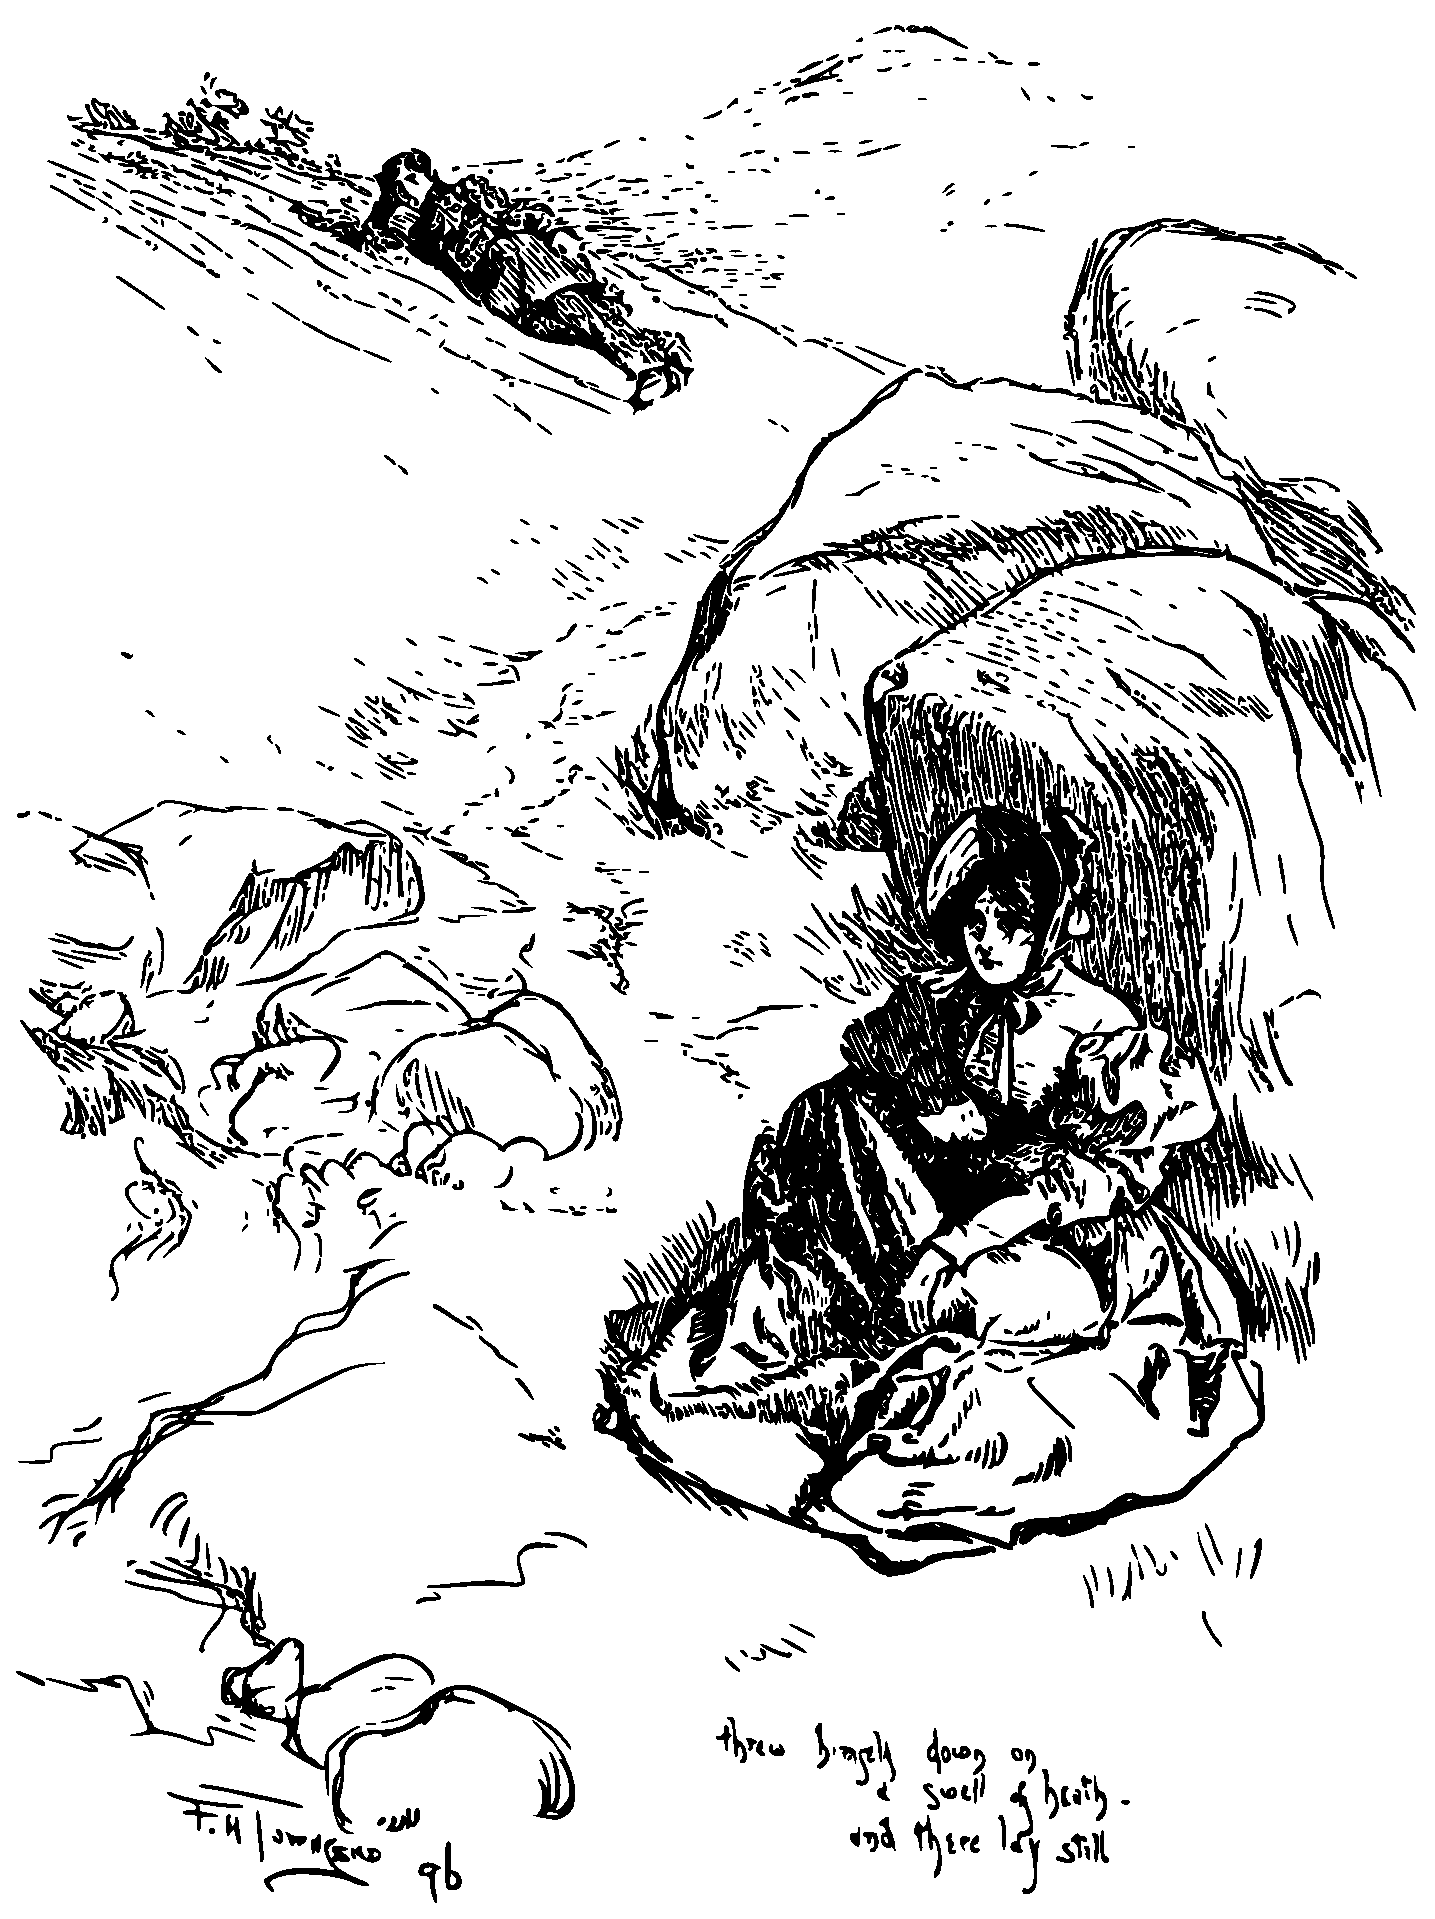
\includegraphics[width=\linewidth]{images/p389b.pdf}
	\end{sidecaption}
\end{figure}

\enquote{I \emph{can} do what he wants me to do: I am forced to see and
acknowledge that,} I meditated,---\enquote{that is, if life be spared me. But
I feel mine is not the existence to be long protracted under an Indian
sun. What then? He does not care for that: when my time came to die,
he would resign me, in all serenity and sanctity, to the God who gave
me. The case is very plain before me. In leaving England, I should
leave a loved but empty land---\Mr{} Rochester is not there; and if he
were, what is, what can that ever be to me? My business is to live
without him now: nothing so absurd, so weak as to drag on from day to
day, as if I were waiting some impossible change in circumstances, which
might reunite me to him. Of course (as \St{} John once said) I must seek
another interest in life to replace the one lost: is not the occupation
he now offers me truly the most glorious man can adopt or God assign? 
Is it not, by its noble cares and sublime results, the one best
calculated to fill the void left by uptorn affections and demolished
hopes? I believe I must say, Yes---and yet I shudder. Alas! If I join
\St{} John, I abandon half myself: if I go to India, I go to premature
death. And how will the interval between leaving England for India, and
India for the grave, be filled? Oh, I know well! That, too, is very
clear to my vision. By straining to satisfy \St{} John till my sinews
ache, I \emph{shall} satisfy him---to the finest central point and
farthest outward circle of his expectations. If I \emph{do} go with
him---if I \emph{do} make the sacrifice he urges, I will make it
absolutely: I will throw all on the altar---heart, vitals, the entire
victim. He will never love me; but he shall approve me; I will show him
energies he has not yet seen, resources he has never suspected. Yes, I
can work as hard as he can, and with as little grudging.

%rem enq
Consent, then, to his demand is possible: but for one
item---one dreadful item. It is---that he asks me to be his wife, and
has no more of a husband's heart for me than that frowning giant of a
rock, down which the stream is foaming in yonder gorge. He prizes me as
a soldier would a good weapon; and that is all. Unmarried to him, this
would never grieve me; but can I let him complete his
calculations---coolly put into practice his plans---go through the
wedding ceremony? Can I receive from him the bridal ring, endure all
the forms of love (which I doubt not he would scrupulously observe) and
know that the spirit was quite absent? Can I bear the consciousness
that every endearment he bestows is a sacrifice made on principle? No:
such a martyrdom would be monstrous. I will never undergo it. As his
sister, I might accompany him---not as his wife: I will tell him so.}

I looked towards the knoll: there he lay, still as a prostrate column;
his face turned to me: his eye beaming watchful and keen. He started to
his feet and approached me.

\enquote{I am ready to go to India, if I may go free.}

\enquote{Your answer requires a commentary,} he said; \enquote{it is not
clear.}

\enquote{You have hitherto been my adopted brother---I, your adopted
sister: let us continue as such: you and I had better not marry.}

He shook his head. \enquote{Adopted fraternity will not do in this
case. If you were my real sister it would be different: I should take
you, and seek no wife. But as it is, either our union must be
consecrated and sealed by marriage, or it cannot exist: practical
obstacles oppose themselves to any other plan. Do you not see it,
Jane? Consider a moment---your strong sense will guide you.}

I did consider; and still my sense, such as it was, directed me only to
the fact that we did not love each other as man and wife should: and
therefore it inferred we ought not to marry. I said so. \enquote{St.
John,} I returned, \enquote{I regard you as a brother---you, me as a
sister: so let us continue.}

\enquote{We cannot---we cannot,} he answered, with short, sharp
determination: \enquote{it would not do. You have said you will go with
me to India: remember---you have said that.}

\enquote{Conditionally.}

\enquote{Well---well. To the main point---the departure with me from
England, the co-operation with me in my future labours---you do not
object. You have already as good as put your hand to the plough: you
are too consistent to withdraw it. You have but one end to keep in
view---how the work you have undertaken can best be done. Simplify your
complicated interests, feelings, thoughts, wishes, aims; merge all
considerations in one purpose: that of fulfilling with effect---with
power---the mission of your great Master. To do so, you must have a
coadjutor: not a brother---that is a loose tie---but a husband. I, too,
do not want a sister: a sister might any day be taken from me. I want a
wife: the sole helpmeet I can influence efficiently in life, and retain
absolutely till death.}

I shuddered as he spoke: I felt his influence in my marrow---his hold on
my limbs.

\enquote{Seek one elsewhere than in me, \St{} John: seek one fitted to
you.}

\enquote{One fitted to my purpose, you mean---fitted to my vocation. 
Again I tell you it is not the insignificant private individual---the
mere man, with the man's selfish senses---I wish to mate: it is the
missionary.}

\enquote{And I will give the missionary my energies---it is all he
wants---but not myself: that would be only adding the husk and shell to
the kernel. For them he has no use: I retain them.}

\enquote{You cannot---you ought not. Do you think God will be satisfied
with half an oblation? Will He accept a mutilated sacrifice? It is the
cause of God I advocate: it is under His standard I enlist you. I
cannot accept on His behalf a divided allegiance: it must be entire.}

\enquote{Oh! I will give my heart to God,} I said. \enquote{\emph{You} do not
want it.}

I will not swear, reader, that there was not something of repressed
sarcasm both in the tone in which I uttered this sentence, and in the
feeling that accompanied it. I had silently feared \St{} John till now,
because I had not understood him. He had held me in awe, because he had
held me in doubt. How much of him was saint, how much mortal, I could
not heretofore tell: but revelations were being made in this conference:
the analysis of his nature was proceeding before my eyes. I saw his
fallibilities: I comprehended them. I understood that, sitting there
where I did, on the bank of heath, and with that handsome form before
me, I sat at the feet of a man, caring as I\@. The veil fell from his
hardness and despotism. Having felt in him the presence of these
qualities, I felt his imperfection and took courage. I was with an
equal---one with whom I might argue---one whom, if I saw good, I might
resist.

He was silent after I had uttered the last sentence, and I presently
risked an upward glance at his countenance.

His eye, bent on me, expressed at once stern surprise and keen inquiry. 
\enquote{Is she sarcastic, and sarcastic to \emph{me}!} it seemed to say. 
\enquote{What does this signify?}

\enquote{Do not let us forget that this is a solemn matter,} he said ere
long; \enquote{one of which we may neither think nor talk lightly
without sin. I trust, Jane, you are in earnest when you say you will
serve your heart to God: it is all I want. Once wrench your heart from
man, and fix it on your Maker, the advancement of that Maker's spiritual
kingdom on earth will be your chief delight and endeavour; you will be
ready to do at once whatever furthers that end. You will see what
impetus would be given to your efforts and mine by our physical and
mental union in marriage: the only union that gives a character of
permanent conformity to the destinies and designs of human beings; and,
passing over all minor caprices---all trivial difficulties and
delicacies of feeling---all scruple about the degree, kind, strength or
tenderness of mere personal inclination---you will hasten to enter into
that union at once.}

\enquote{Shall I?} I said briefly; and I looked at his features,
beautiful in their harmony, but strangely formidable in their still
severity; at his brow, commanding but not open; at his eyes, bright and
deep and searching, but never soft; at his tall imposing figure; and
fancied myself in idea \emph{his wife}. Oh! it would never do! As his
curate, his comrade, all would be right: I would cross oceans with him
in that capacity; toil under Eastern suns, in Asian deserts with him in
that office; admire and emulate his courage and devotion and vigour;
accommodate quietly to his masterhood; smile undisturbed at his
ineradicable ambition; discriminate the Christian from the man:
profoundly esteem the one, and freely forgive the other. I should
suffer often, no doubt, attached to him only in this capacity: my body
would be under rather a stringent yoke, but my heart and mind would be
free. I should still have my unblighted self to turn to: my natural
unenslaved feelings with which to communicate in moments of loneliness. 
There would be recesses in my mind which would be only mine, to which he
never came, and sentiments growing there fresh and sheltered which his
austerity could never blight, nor his measured warrior-march trample
down: but as his wife---at his side always, and always restrained, and
always checked---forced to keep the fire of my nature continually low,
to compel it to burn inwardly and never utter a cry, though the
imprisoned flame consumed vital after vital---\emph{this} would be
unendurable.

\enquote{\St{} John!} I exclaimed, when I had got so far in my meditation.

\enquote{Well?} he answered icily.

\enquote{I repeat I freely consent to go with you as your
fellow-missionary, but not as your wife; I cannot marry you and become
part of you.}

\enquote{A part of me you must become,} he answered steadily;
\enquote{otherwise the whole bargain is void. How can I, a man not yet
thirty, take out with me to India a girl of nineteen, unless she be
married to me? How can we be for ever together---sometimes in
solitudes, sometimes amidst savage tribes---and unwed?}

\enquote{Very well,} I said shortly; \enquote{under the circumstances,
quite as well as if I were either your real sister, or a man and a
clergyman like yourself.}

\enquote{It is known that you are not my sister; I cannot introduce you
as such: to attempt it would be to fasten injurious suspicions on us
both. And for the rest, though you have a man's vigorous brain, you
have a woman's heart and---it would not do.}

\enquote{It would do,} I affirmed with some disdain, \enquote{perfectly
well. I have a woman's heart, but not where you are concerned; for you
I have only a comrade's constancy; a fellow-soldier's frankness,
fidelity, fraternity, if you like; a neophyte's respect and submission
to his hierophant: nothing more---don't fear.}

\enquote{It is what I want,} he said, speaking to himself; \enquote{it is just
what I want. And there are obstacles in the way: they must be hewn
down. Jane, you would not repent marrying me---be certain of that; we
\emph{must} be married. I repeat it: there is no other way; and
undoubtedly enough of love would follow upon marriage to render the
union right even in your eyes.}

\enquote{I scorn your idea of love,} I could not help saying, as I rose
up and stood before him, leaning my back against the rock. \enquote{I
scorn the counterfeit sentiment you offer: yes, \St{} John, and I scorn
you when you offer it.}

He looked at me fixedly, compressing his well-cut lips while he did so. 
Whether he was incensed or surprised, or what, it was not easy to tell:
he could command his countenance thoroughly.

\enquote{I scarcely expected to hear that expression from you,} he said:
\enquote{I think I have done and uttered nothing to deserve scorn.}

I was touched by his gentle tone, and overawed by his high, calm mien.

\enquote{Forgive me the words, \St{} John; but it is your own fault that I
have been roused to speak so unguardedly. You have introduced a topic
on which our natures are at variance---a topic we should never discuss:
the very name of love is an apple of discord between us. If the reality
were required, what should we do? How should we feel? My dear cousin,
abandon your scheme of marriage---forget it.}

\enquote{No,} said he; \enquote{it is a long-cherished scheme, and the
only one which can secure my great end: but I shall urge you no further
at present. To-morrow, I leave home for Cambridge: I have many friends
there to whom I should wish to say farewell. I shall be absent a
fortnight---take that space of time to consider my offer: and do not
forget that if you reject it, it is not me you deny, but God. Through
my means, He opens to you a noble career; as my wife only can you enter
upon it. Refuse to be my wife, and you limit yourself for ever to a
track of selfish ease and barren obscurity. Tremble lest in that case
you should be numbered with those who have denied the faith, and are
worse than infidels!}

He had done. Turning from me, he once more

\settoversewidth{\versewidth}{'Looked to river, looked to hill.'}
\begin{verse}[\versewidth]
\enquote{Looked to river, looked to hill.}
\end{verse}

But this time his feelings were all pent in his heart: I was not worthy
to hear them uttered. As I walked by his side homeward, I read well in
his iron silence all he felt towards me: the disappointment of an
austere and despotic nature, which has met resistance where it expected
submission---the disapprobation of a cool, inflexible judgment, which
has detected in another feelings and views in which it has no power to
sympathise: in short, as a man, he would have wished to coerce me into
obedience: it was only as a sincere Christian he bore so patiently with
my perversity, and allowed so long a space for reflection and
repentance.

That night, after he had kissed his sisters, he thought proper to forget
even to shake hands with me, but left the room in silence. I---who,
though I had no love, had much friendship for him---was hurt by the
marked omission: so much hurt that tears started to my eyes.

\enquote{I see you and \St{} John have been quarrelling, Jane,} said
Diana, \enquote{during your walk on the moor. But go after him; he is
now lingering in the passage expecting you---he will make it up.}

I have not much pride under such circumstances: I would always rather be
happy than dignified; and I ran after him---he stood at the foot of the
stairs.

\enquote{Good-night, \St{} John,} said I\@.

\enquote{Good-night, Jane,} he replied calmly.

\enquote{Then shake hands,} I added.

What a cold, loose touch, he impressed on my fingers! He was deeply
displeased by what had occurred that day; cordiality would not warm, nor
tears move him. No happy reconciliation was to be had with him---no
cheering smile or generous word: but still the Christian was patient and
placid; and when I asked him if he forgave me, he answered that he was
not in the habit of cherishing the remembrance of vexation; that he had
nothing to forgive, not having been offended.

And with that answer he left me. I would much rather he had knocked me
down.
